\chapter{An�lisis}
En este cap�tulo se proceder� a la descomposici�n del dominio en el que trabaja la aplicaci�n. De esta manera, se podr�n identificar los distintos casos de uso que debe abordar la misma para cubrir las distintas necesidades de los usuarios. \\
Es necesario distinguir previamente dos tipos de perfil de usuario que tendr�n a su disposici�n distintas funcionalidades del sistema. Estos dos tipos son el usuario no autenticado y el usuario autenticado, los cuales difieren �nicamente en que el segundo est� vinculado a una cuenta de usuario y dispone, por tanto, de todas las operaciones relativas a la cuenta. \\
En la figura~\ref{fig:CasosUso} se muestran los distintos casos de uso que se identificaron en la aplicaci�n.

\begin{figure}[htbp]
	\centering
		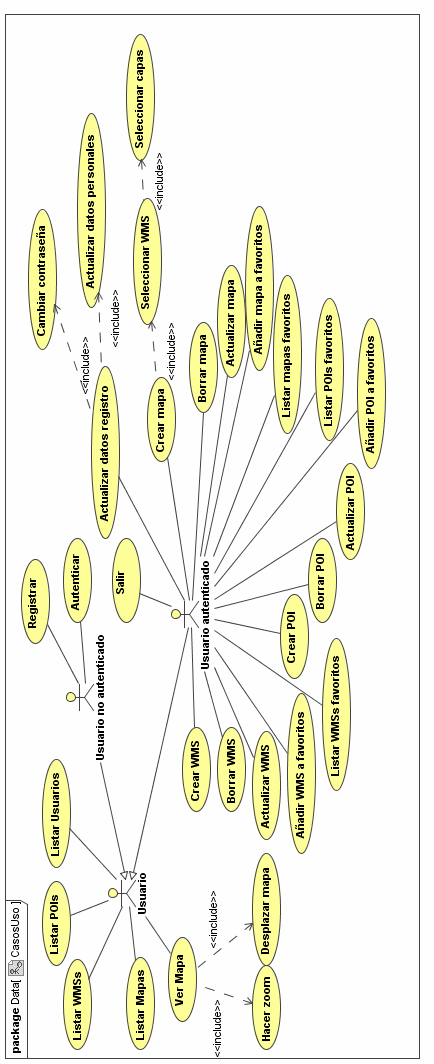
\includegraphics[scale=0.5]{Im�genes/CasosUso.png}
	\caption{Casos de uso de la aplicaci�n}
	\label{fig:CasosUso}
\end{figure}
